\documentclass[tikz,border=6pt]{standalone}
\usepackage{amsmath,amssymb}
\usetikzlibrary{decorations.markings,arrows.meta,calc}

% ---------------- 只保留两种核心颜色 ----------------
\definecolor{loopF}{RGB}{30,100,190}      % 颜色一：深蓝色 (代表味道 f)
\definecolor{loopOther}{RGB}{220,70,70}   % 颜色二：珊瑚红 (代表其他味道)

\begin{document}

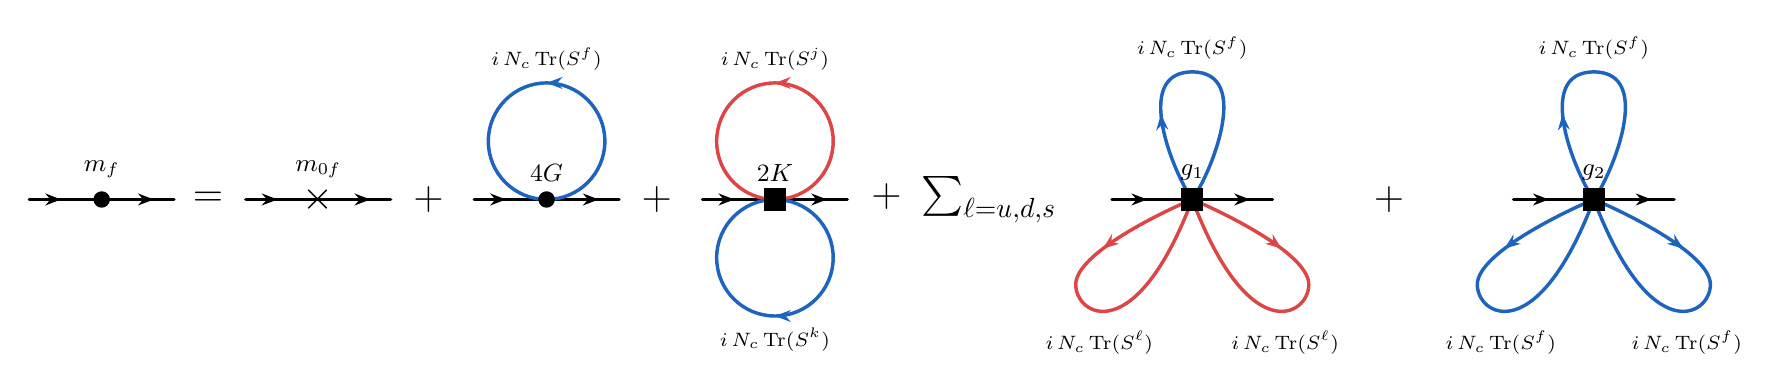
\begin{tikzpicture}[
    x=1cm,y=1cm,
    line cap=round,
    line join=round,
    every node/.style={font=\small},
    prop/.style={
        line width=1.15pt,
        postaction={decorate},
        decoration={markings,
            mark=at position 0.22 with {\arrow{Stealth[length=2.0mm,width=1.5mm]}},
            mark=at position 0.86 with {\arrow{Stealth[length=2.0mm,width=1.5mm]}}
        }
    },
    looptop/.style={
        line width=1.25pt,
        postaction={decorate},
        decoration={markings,
            mark=at position 0.50 with {\arrow{Stealth[length=2.0mm,width=1.5mm]}}
        }
    },
    petaltop/.style={
        line width=1.25pt,
        postaction={decorate},
        decoration={markings,
            mark=at position 0.30 with {\arrow{Stealth[length=2.0mm,width=1.5mm]}}
        }
    },
    petalleft/.style={
        line width=1.25pt,
        postaction={decorate},
        decoration={markings,
            mark=at position 0.30 with {\arrow{Stealth[length=2.0mm,width=1.5mm]}}
        }
    },
    petalright/.style={
        line width=1.25pt,
        postaction={decorate},
        decoration={markings,
            mark=at position 0.30 with {\arrow{Stealth[length=2.0mm,width=1.5mm]}}
        }
    },
    vdot/.style={circle,fill=black,inner sep=2.1pt},
    vsq/.style={
        rectangle,
        fill=black,
        minimum width=8pt,
        minimum height=8pt,
        inner sep=0pt
    },
    lab/.style={font=\small},
    looplab/.style={font=\scriptsize}
]

% ============================================================
% 4q and 6q loops
% ============================================================

\newcommand{\TopCircleLoop}[2]{%
    \draw[looptop,draw=#1]
        (0,0) arc[start angle=-90,end angle=270,radius=0.74];
    \node[looplab] at (0,1.78) {#2};
}

\newcommand{\BottomCircleLoop}[2]{%
    \draw[looptop,draw=#1]
        (0,0) arc[start angle=90,end angle=-270,radius=0.74];
    \node[looplab] at (0,-1.78) {#2};
}
% ============================================================
% 8q smooth three-petal loops: no cusp at the outer tip
% ============================================================

\newcommand{\TopPetalLoop}[2]{%
    \draw[petaltop,draw=#1]
        (0,0)
        .. controls (-0.22,0.30) and (-0.78,1.62) .. (0,1.62)
        .. controls ( 0.78,1.62) and ( 0.22,0.30) .. (0,0);
    \node[looplab] at (0,1.92) {#2};
}

\newcommand{\LeftPetalLoop}[2]{%
    \draw[petalleft,draw=#1]
        (0,0)
        .. controls (-0.34,-0.14) and (-1.48,-0.68) .. (-1.48,-1.08)
        .. controls (-1.48,-1.48) and (-0.72,-1.90) .. (0,0);
    \node[looplab] at (-1.18,-1.82) {#2};
}

\newcommand{\RightPetalLoop}[2]{%
    \draw[petalright,draw=#1]
        (0,0)
        .. controls (0.34,-0.14) and (1.48,-0.68) .. (1.48,-1.08)
        .. controls (1.48,-1.48) and (0.72,-1.90) .. (0,0);
    \node[looplab] at (1.18,-1.82) {#2};
}
% ============================================================
% m_f
% ============================================================

\begin{scope}[shift={(0,0)}]
    \draw[prop] (-0.92,0) -- (0.92,0);
    \node[vdot] at (0,0) {};
    \node[lab] at (0,0.38) {$m_f$};
\end{scope}

\node[font=\Large] at (1.35,0) {$=$};

% ============================================================
% m_{0f}
% ============================================================

\begin{scope}[shift={(2.75,0)}]
    \draw[prop] (-0.92,0) -- (0.92,0);
    \node[font=\Large] at (0,0) {$\times$};
    \node[lab] at (0,0.38) {$m_{0f}$};
\end{scope}

\node[font=\Large] at (4.15,0) {$+$};

% ============================================================
% 4-quark term
% ============================================================

\begin{scope}[shift={(5.65,0)}]
    \draw[prop] (-0.92,0) -- (0.92,0);

    \TopCircleLoop{loopF}
    {$i\,N_c\,\mathrm{Tr}(S^{f})$}

    \node[vdot] at (0,0) {};
    \node[lab] at (0,0.34) {$4G$};
\end{scope}

\node[font=\Large] at (7.05,0) {$+$};

% ============================================================
% 6-quark term
% ============================================================

\begin{scope}[shift={(8.55,0)}]
    \draw[prop] (-0.92,0) -- (0.92,0);

    \TopCircleLoop{loopOther}
    {$i\,N_c\,\mathrm{Tr}(S^{j})$}

    \BottomCircleLoop{loopF}
    {$i\,N_c\,\mathrm{Tr}(S^{k})$}

    \node[vsq] at (0,0) {};
    \node[lab] at (0,0.34) {$2K$};
\end{scope}

\node[font=\Large] at (10.95,0) {$+\ \sum_{\ell=u,d,s}$};

% ============================================================
% 8-quark g1 term
% ============================================================

\begin{scope}[shift={(13.85,0)}]
    \draw[prop] (-1.02,0) -- (1.02,0);

    \TopPetalLoop{loopF}
    {$i\,N_c\,\mathrm{Tr}(S^{f})$}

    \LeftPetalLoop{loopOther}
    {$i\,N_c\,\mathrm{Tr}(S^{\ell})$}

    \RightPetalLoop{loopOther}
    {$i\,N_c\,\mathrm{Tr}(S^{\ell})$}

    \node[vsq] at (0,0) {};
    \node[lab] at (0,0.34) {$g_1$};
\end{scope}

\node[font=\Large] at (16.35,0) {$+$};

% ============================================================
% 8-quark g2 term
% ============================================================

\begin{scope}[shift={(18.95,0)}]
    \draw[prop] (-1.02,0) -- (1.02,0);

    \TopPetalLoop{loopF}
    {$i\,N_c\,\mathrm{Tr}(S^{f})$}

    \LeftPetalLoop{loopF}
    {$i\,N_c\,\mathrm{Tr}(S^{f})$}

    \RightPetalLoop{loopF}
    {$i\,N_c\,\mathrm{Tr}(S^{f})$}

    \node[vsq] at (0,0) {};
    \node[lab] at (0,0.34) {$g_2$};
\end{scope}

\end{tikzpicture}

\end{document}